\subsection{Desenvolvimento do Tratamento}

A nova versão do produto foi implementada com a adição de uma condicional no código para definir a posição do filtro de nível de dificuldade. Essa condicional foi vinculada a um \textit{feature gate} denominado \textit{experiment/difficulty-filter-position} (como descrito na Subseção \ref{subsubsec:variants}). 

Na tela de criação de listas de exercícios, os três primeiros filtros são essenciais para determinados casos de uso do produto. Por essa razão, por decisão estratégica, o filtro de nível de dificuldade foi elevado apenas até a quarta posição, garantindo que fluxos críticos não fossem impactados. O trecho de código a seguir ilustra uma implementação semelhante à utilizada na versão de tratamento.

\vspace{\onelineskip}
\begin{lstlisting}[style=customJS]
function FiltersComponent() {
    const isFiltersOrderExperimentEnabled = useFeature(
        'experiment/difficulty-filter-position'
    );

    return (
      <div>
        {otherFilter1}
        {otherFilter2}
        {otherFilter3}
        {isFiltersOrderExperimentEnabled 
            ? estimatedDifficultyFilter 
            : null}
        {otherFilter4}
        {otherFilter5}
        {otherFilter6}
        {otherFilter7}
        {isFiltersOrderExperimentEnabled 
            ? null 
            : estimatedDifficultyFilter}
      </div>
    );
}
\end{lstlisting}


Finalizado o desenvolvimento, seguindo o fluxo padrão da empresa para a liberação de novas versões, o código passou por revisão e análise. Após a realização da \textit{release}, a versão de tratamento foi ativada exclusivamente para os usuários beta, iniciando assim a coleta de dados.  É importante destacar que, embora as escolas beta estejam cientes de que podem receber versões experimentais do produto ou funcionalidades em desenvolvimento, nenhum usuário foi informado sobre este experimento, evitando assim possíveis vieses em seu comportamento.




\subsection{Execução do Experimento}
\label{subsec:experimento}

Os dados de uso das diferentes versões da funcionalidade foram coletados ao longo de um período de duas semanas, de 5 a 18 de novembro de 2024. Durante esse intervalo, foram registrados 80.198 eventos de filtragem e 30.731 listas de exercícios criadas. O primeiro passo da análise consistiu na segmentação dos usuários únicos, focando inicialmente na utilização do filtro de nível de dificuldade. Para evitar distorções nas medidas de tendência central, foram excluídos do conjunto de dados os usuários que não utilizaram o filtro em nenhuma ocasião, uma vez que representavam 85\% da amostra observada.

Após essa filtragem inicial, o conjunto original de 3.504 docentes foi reduzido para 517 usuários, dos quais 429 ($\approx$83\%) pertenciam ao grupo de controle e 88 ($\approx$17\%) ao grupo de tratamento. Para essa amostra, foram extraídas métricas referentes ao número de listas de exercícios criadas e à quantidade de questões selecionadas no período analisado. Em seguida, foram aplicadas técnicas de estatística descritiva para compreender o comportamento dos usuários, incluindo a análise de diagramas de caixa e medidas de tendência central.

Num primeiro momentou, observou-se uma quantidade considerável de \textit{outliers} nos conjuntos coletados (tanto para as métricas de filtros quanto para as métricas de listas e exercícios), tornando necessária a aplicação do método do intervalo interquartil para sua remoção. Esse método foi escolhido por ser adequado a conjuntos de dados que não seguem uma distribuição normal (o processo é melhor detalhado na Subseção \ref{subsec:reduction}). Este procedimento resultou na exclusão de 78 \textit{outliers}, fazendo com que a amostra final passasse a contar com 439 usuários, sendo 363 ($\approx$83\%) do grupo de controle e 76 ($\approx$17\%) do grupo de tratamento.

Com relação ao número de usos do filtro, os gráficos de caixa de antes e depois da remoção dos \textit{outliers} são apresentados, respectivamente, nas Figuras \ref{fig:box-uses-before} e \ref{fig:box-uses-after}. Além disso, as medidas de tendência central podem ser verificadas nas Figuras \ref{fig:mtc-uses-before} e \ref{fig:mtc-uses-after}.

\begin{figure}
    \centering
    \caption{Gráfico de Caixa do Número de Usos do Filtro Antes da Remoção de \textit{Outliers}}
    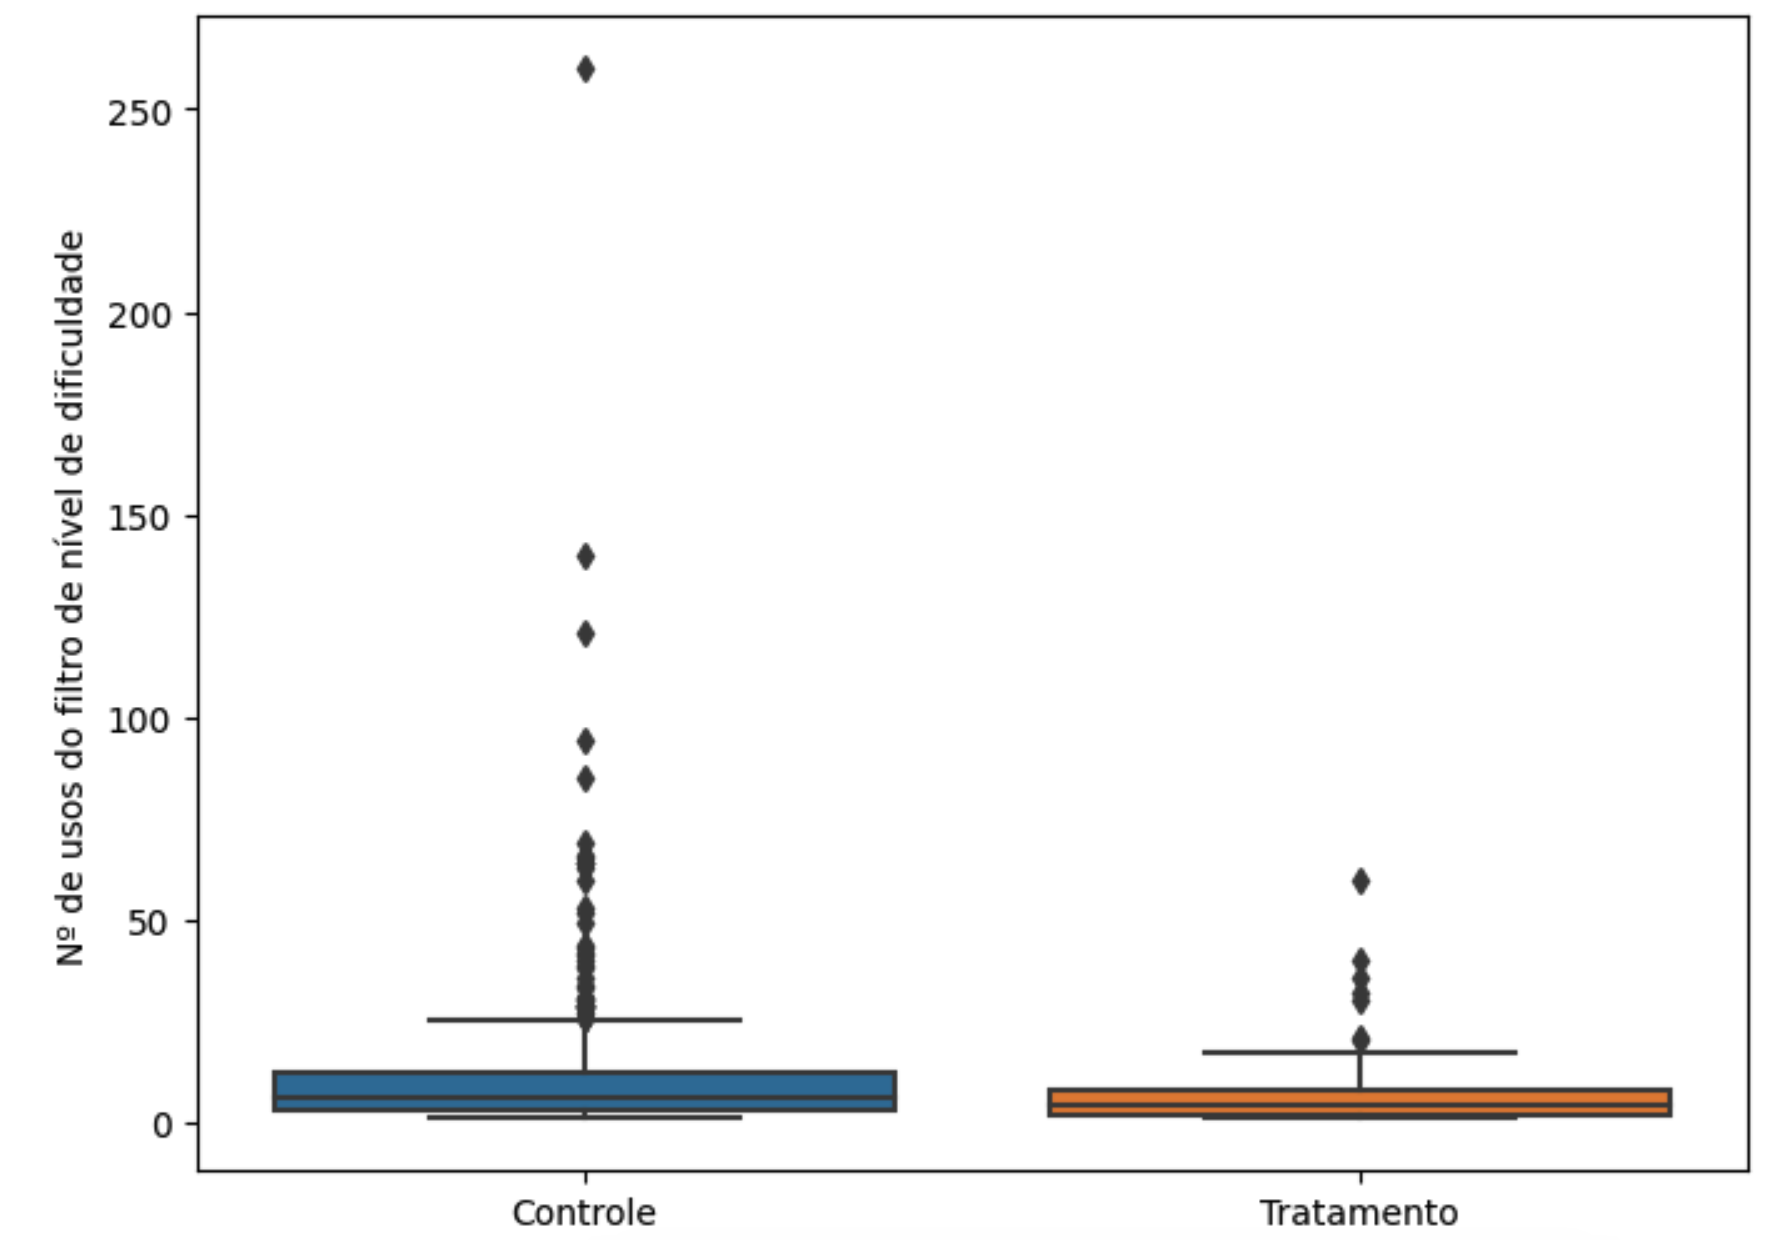
\includegraphics[width=0.85\linewidth]{figuras/boxplot_uses_before.png}
    \begin{center}
        \text{Fonte: Autor}
    \end{center}
    \label{fig:box-uses-before}
\end{figure}

\begin{figure}
    \centering
    \caption{Gráfico de Caixa do Número de Usos do Filtro Após Remoção de \textit{Outliers}}
    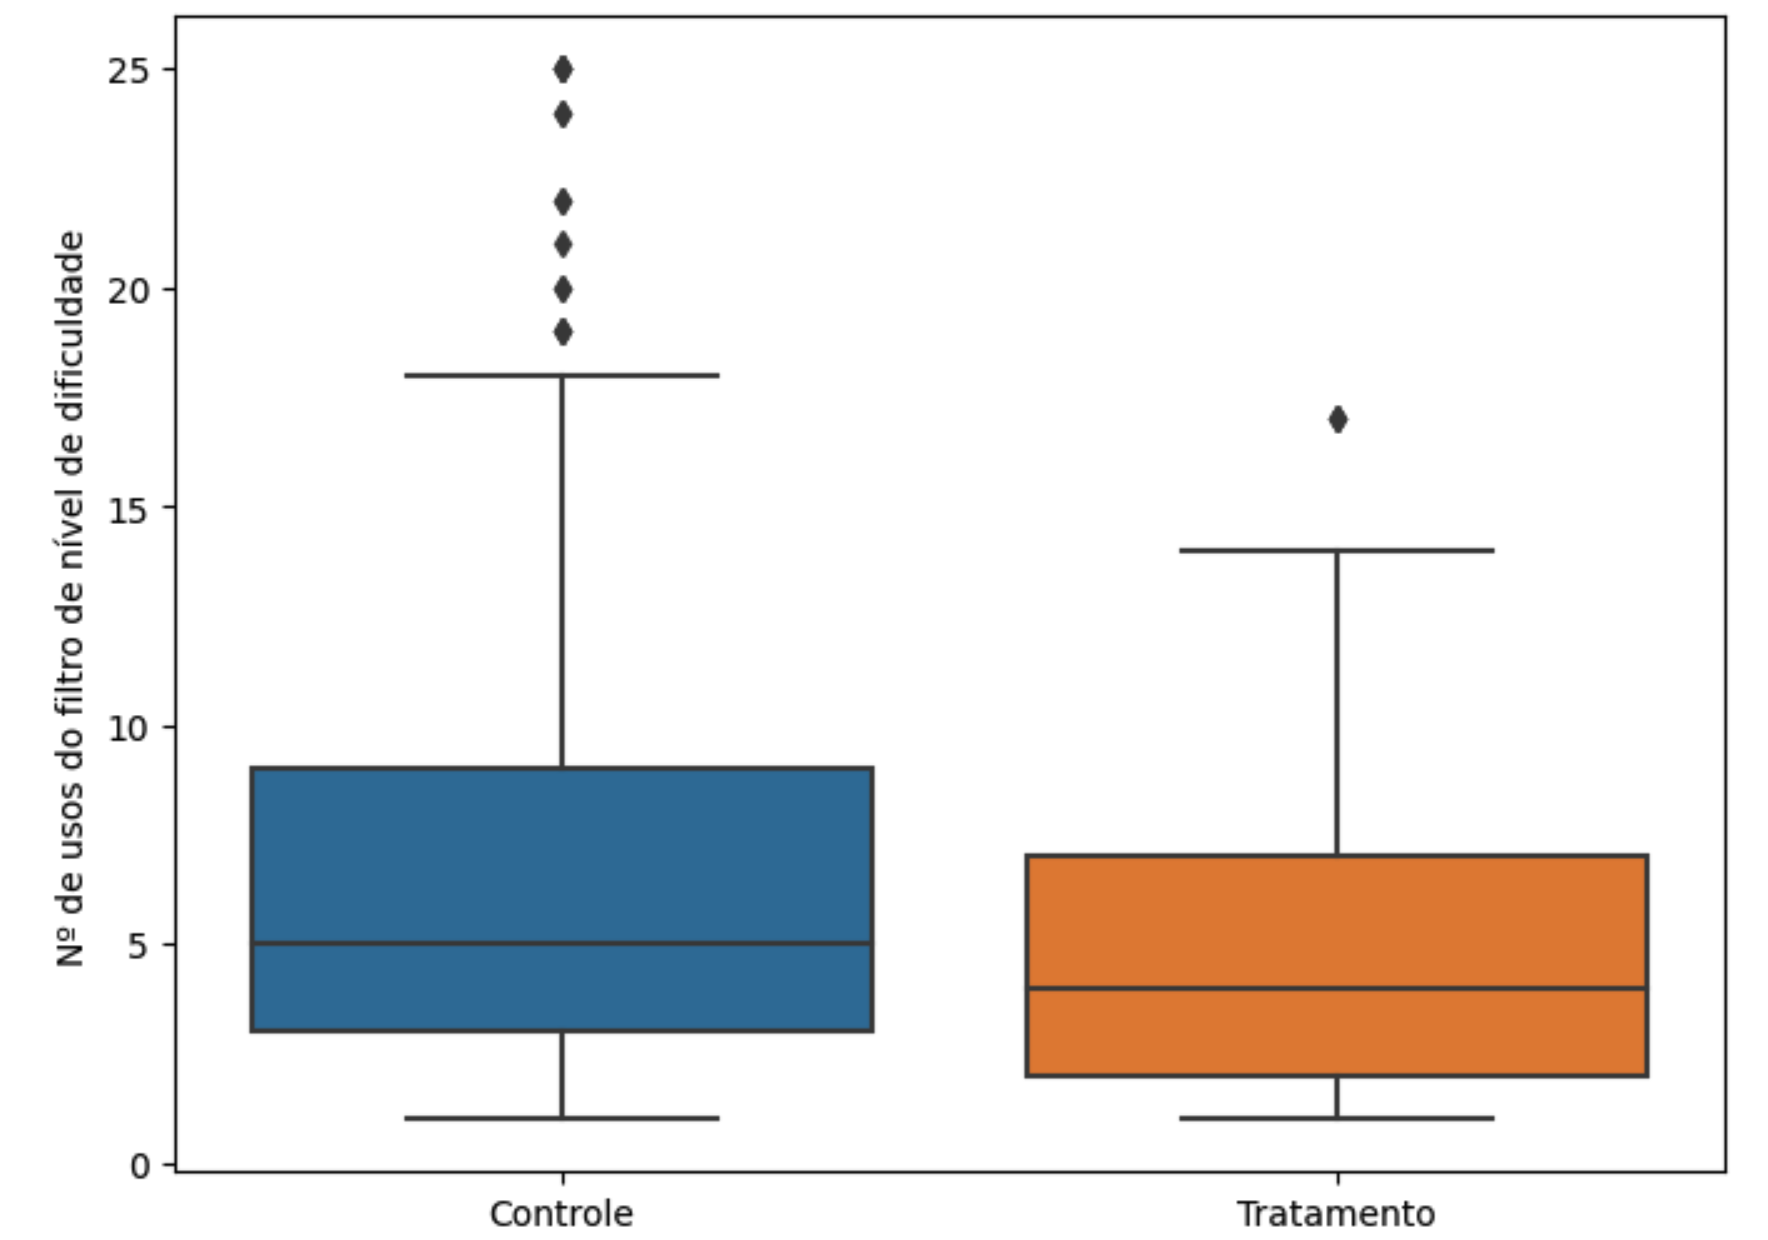
\includegraphics[width=0.85\linewidth]{figuras/boxplot_uses_after.png}
    \begin{center}
        \text{Fonte: Autor}
    \end{center}
    \label{fig:box-uses-after}
\end{figure}

\begin{figure}
    \centering
    \caption{Medidas de Tendência Central do Número de Usos do Filtro Antes da Remoção de \textit{Outliers}}
    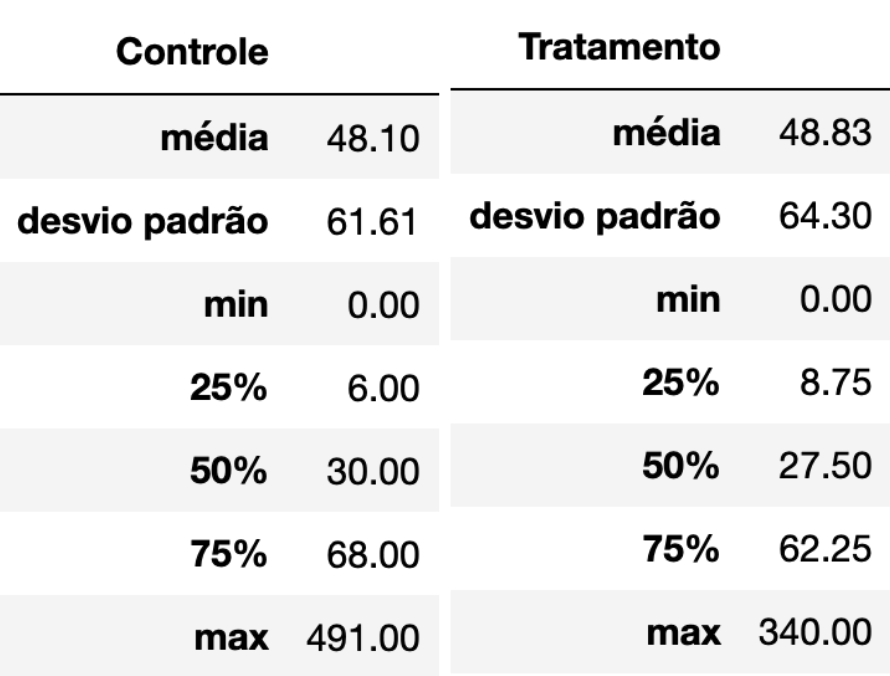
\includegraphics[width=0.45\linewidth]{figuras/mtc_uses_before.png}
    \begin{center}
        \text{Fonte: Autor}
    \end{center}
    \label{fig:mtc-uses-before}
\end{figure}

\begin{figure}
    \centering
    \caption{Medidas de Tendência Central do Número de Usos do Filtro Após Remoção de \textit{Outliers}}
    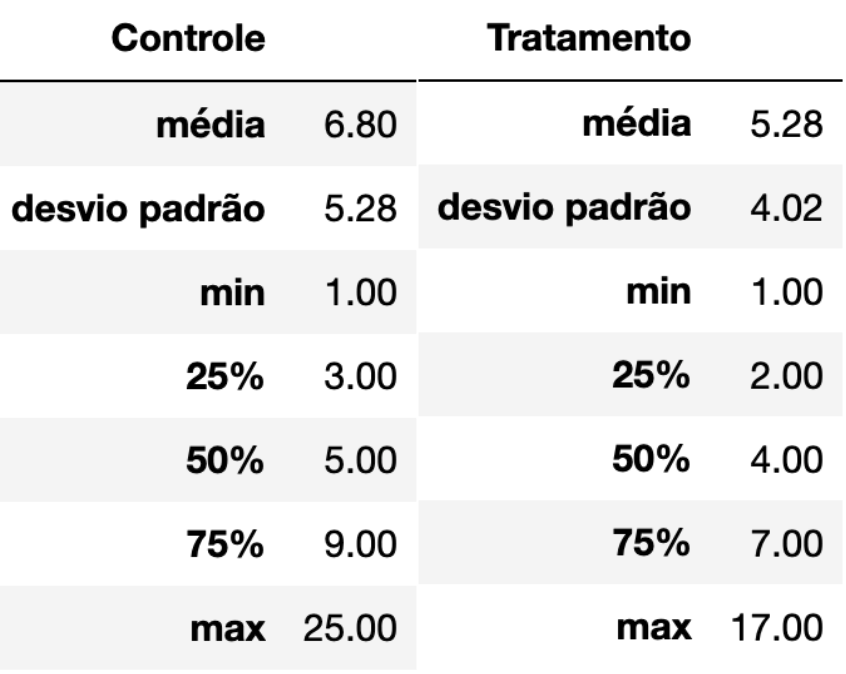
\includegraphics[width=0.45\linewidth]{figuras/mtc_uses_after.png}
    \begin{center}
        \text{Fonte: Autor}
    \end{center}
    \label{fig:mtc-uses-after}
\end{figure}

O mesmo processo foi realizado para o número de listas de exercícios criadas, cujos gráficos de caixa estão disponíveis nas Figuras \ref{fig:box-acts-before} e \ref{fig:box-acts-after}, e as respectivas medidas de tendência central nas Figuras \ref{fig:mtc-acts-before} e \ref{fig:mtc-acts-after}.

\begin{figure}
    \centering
    \caption{Gráfico de Caixa do Número de Listas Criadas Antes da Remoção de \textit{Outliers}}
    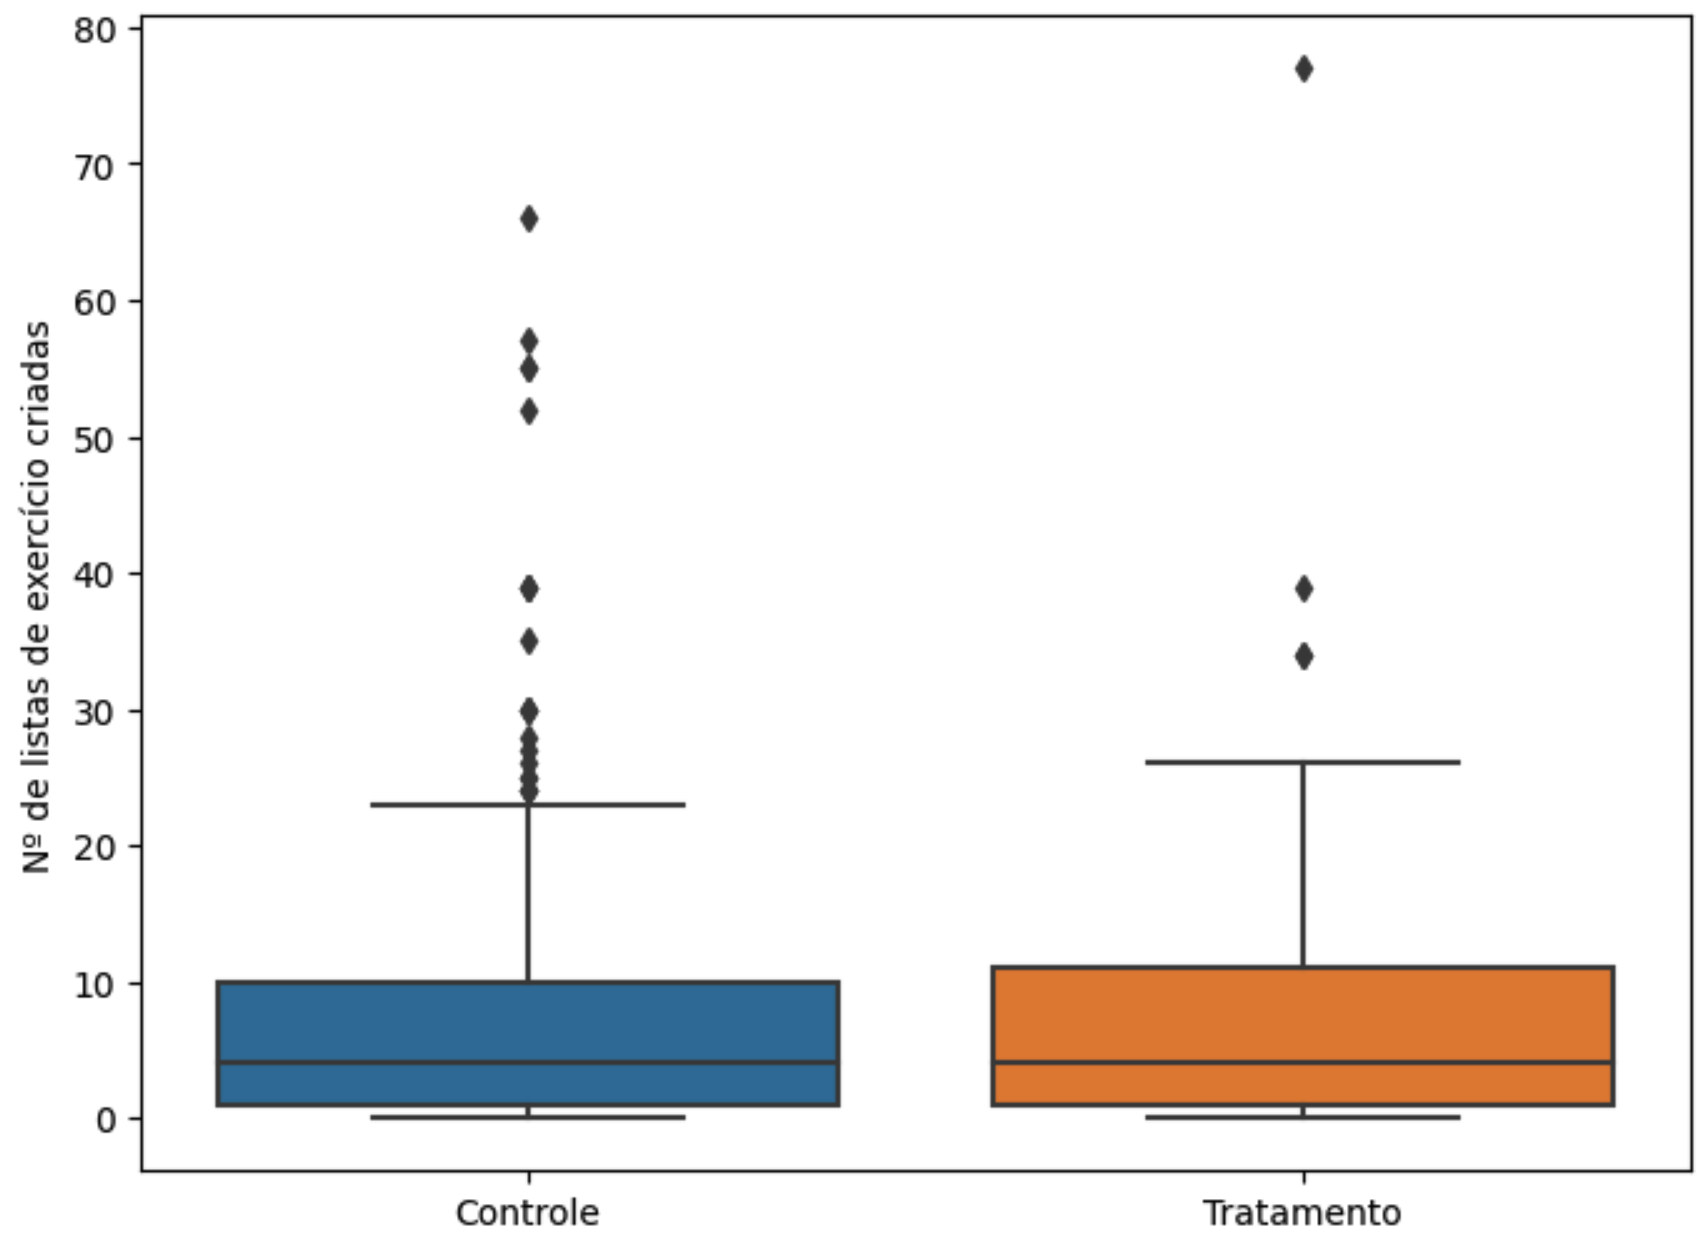
\includegraphics[width=0.85\linewidth]{figuras/boxplot_acts_before.png}
    \begin{center}
        \text{Fonte: Autor}
    \end{center}
    \label{fig:box-acts-before}
\end{figure}

\begin{figure}
    \centering
    \caption{Gráfico de Caixa do Número de Listas Criadas Após Remoção de \textit{Outliers}}
    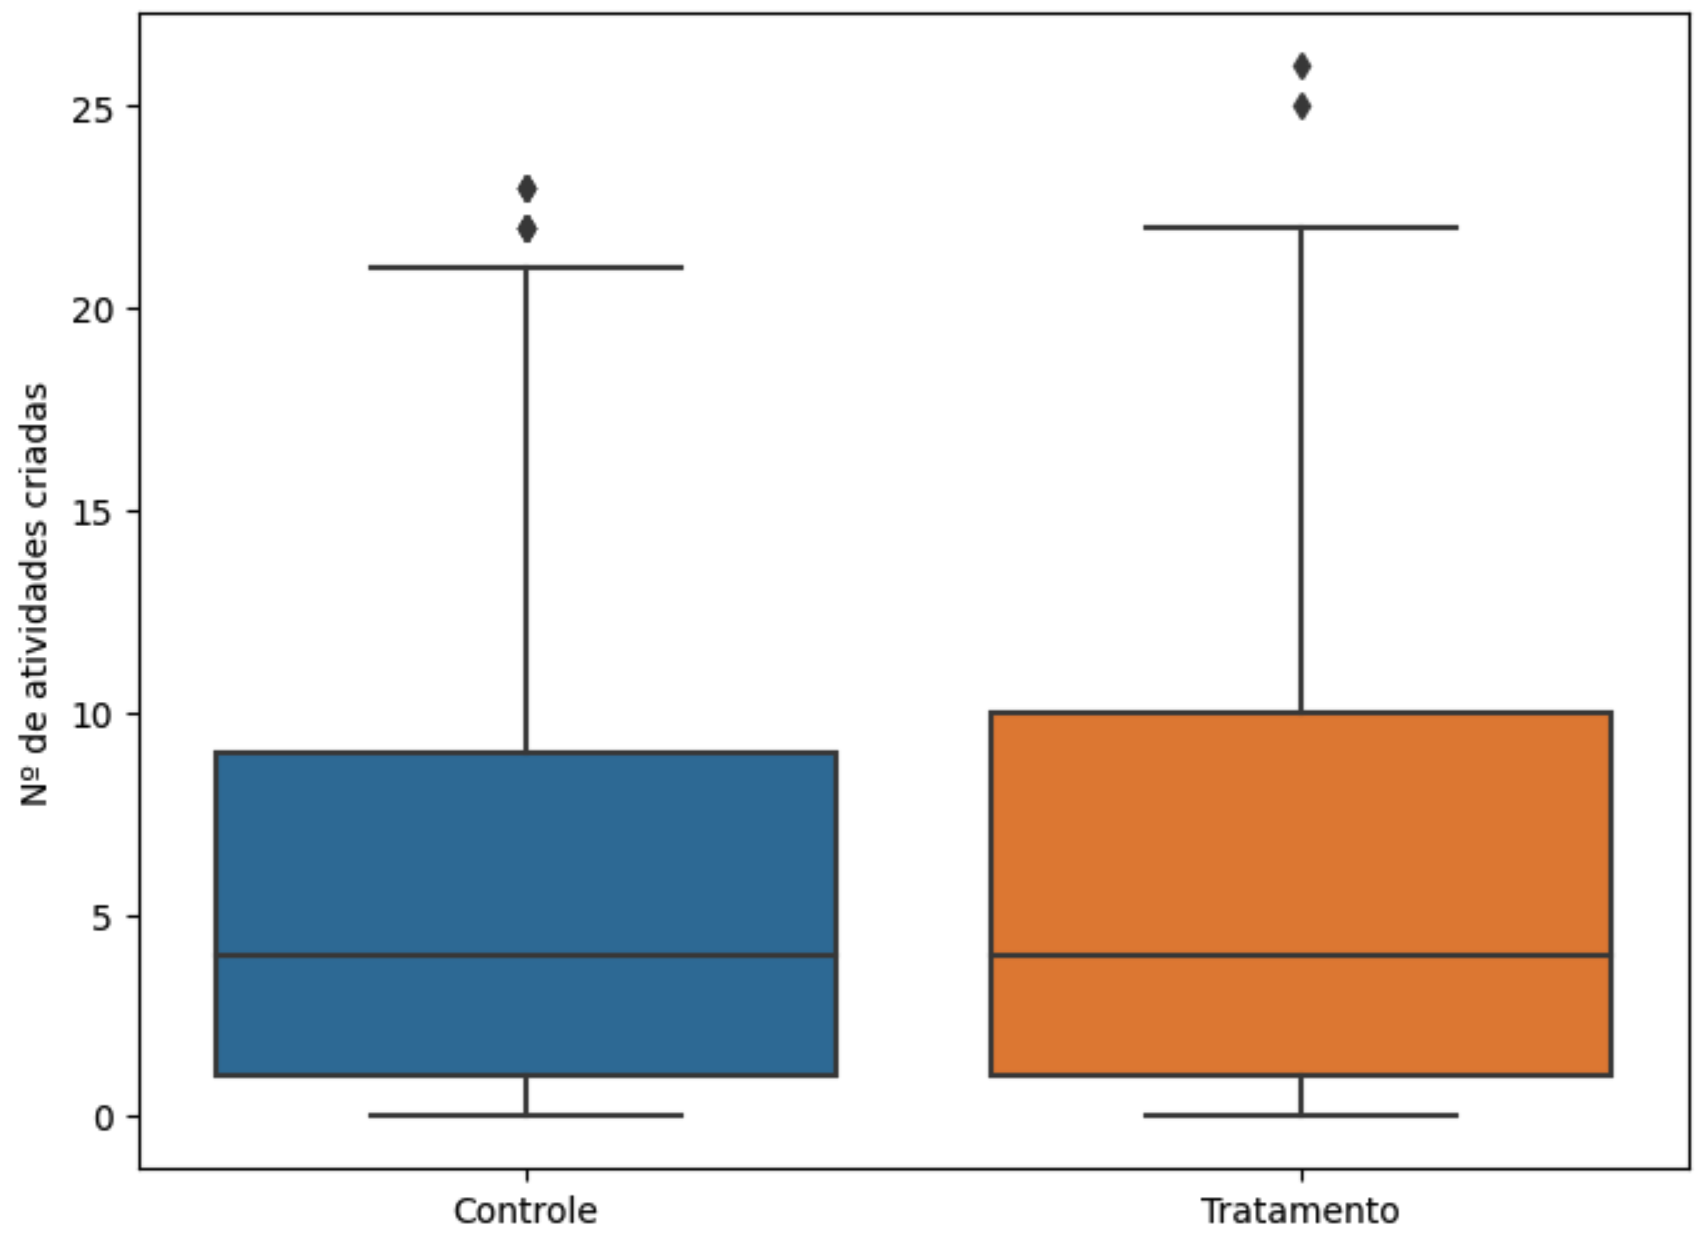
\includegraphics[width=0.85\linewidth]{figuras/boxplot_acts_after.png}
    \begin{center}
        \text{Fonte: Autor}
    \end{center}
    \label{fig:box-acts-after}
\end{figure}

\begin{figure}
    \centering
    \caption{Medidas de Tendência Central do Número de Listas Criadas Antes da Remoção de \textit{Outliers}}
    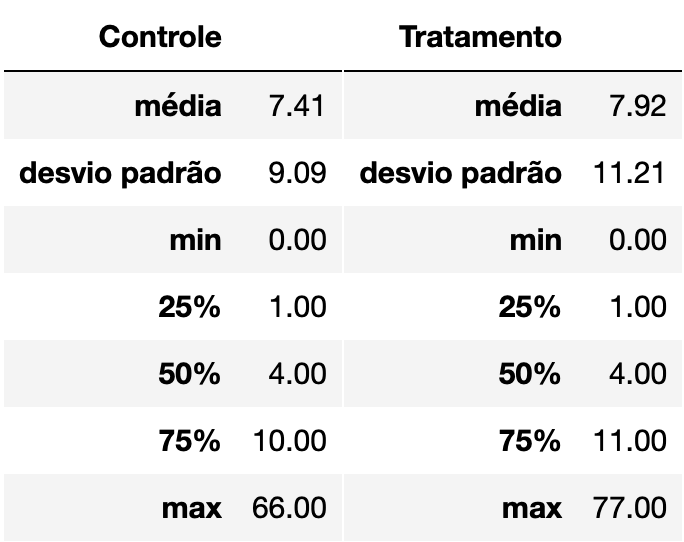
\includegraphics[width=0.45\linewidth]{figuras/mtc_acts_before.png}
    \begin{center}
        \text{Fonte: Autor}
    \end{center}
    \label{fig:mtc-acts-before}
\end{figure}

\begin{figure}
    \centering
    \caption{Medidas de Tendência Central do Número de Listas Criadas Após Remoção de \textit{Outliers}}
    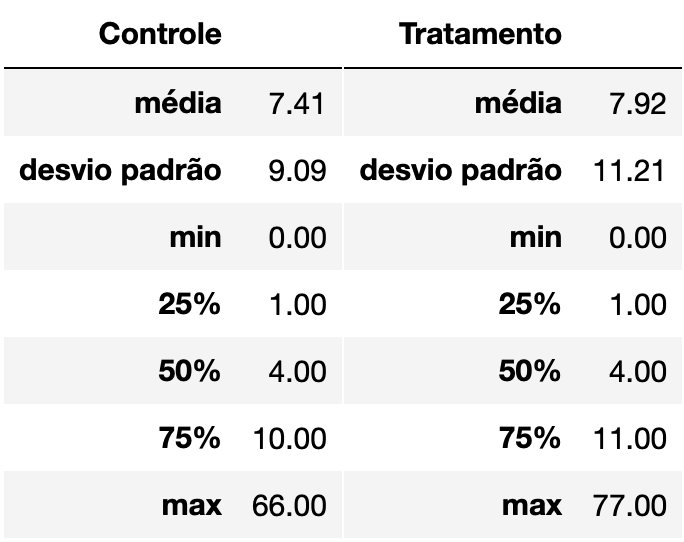
\includegraphics[width=0.45\linewidth]{figuras/mtc_acts_after.png}
    \begin{center}
        \text{Fonte: Autor}
    \end{center}
    \label{fig:mtc-acts-after}
\end{figure}

O mesmo padrão de análise foi seguido para o número de exercícios selecionados, cujos resultados estão ilustrados nas Figuras \ref{fig:box-exs-before} e \ref{fig:box-exs-after} para os gráficos de caixa, e nas Figuras \ref{fig:mtc-exs-before} e \ref{fig:mtc-exs-after} para as medidas de tendência central.

\begin{figure}
    \centering
    \caption{Gráfico de Caixa do Número de Exercícios Selecionados Antes da Remoção de \textit{Outliers}}
    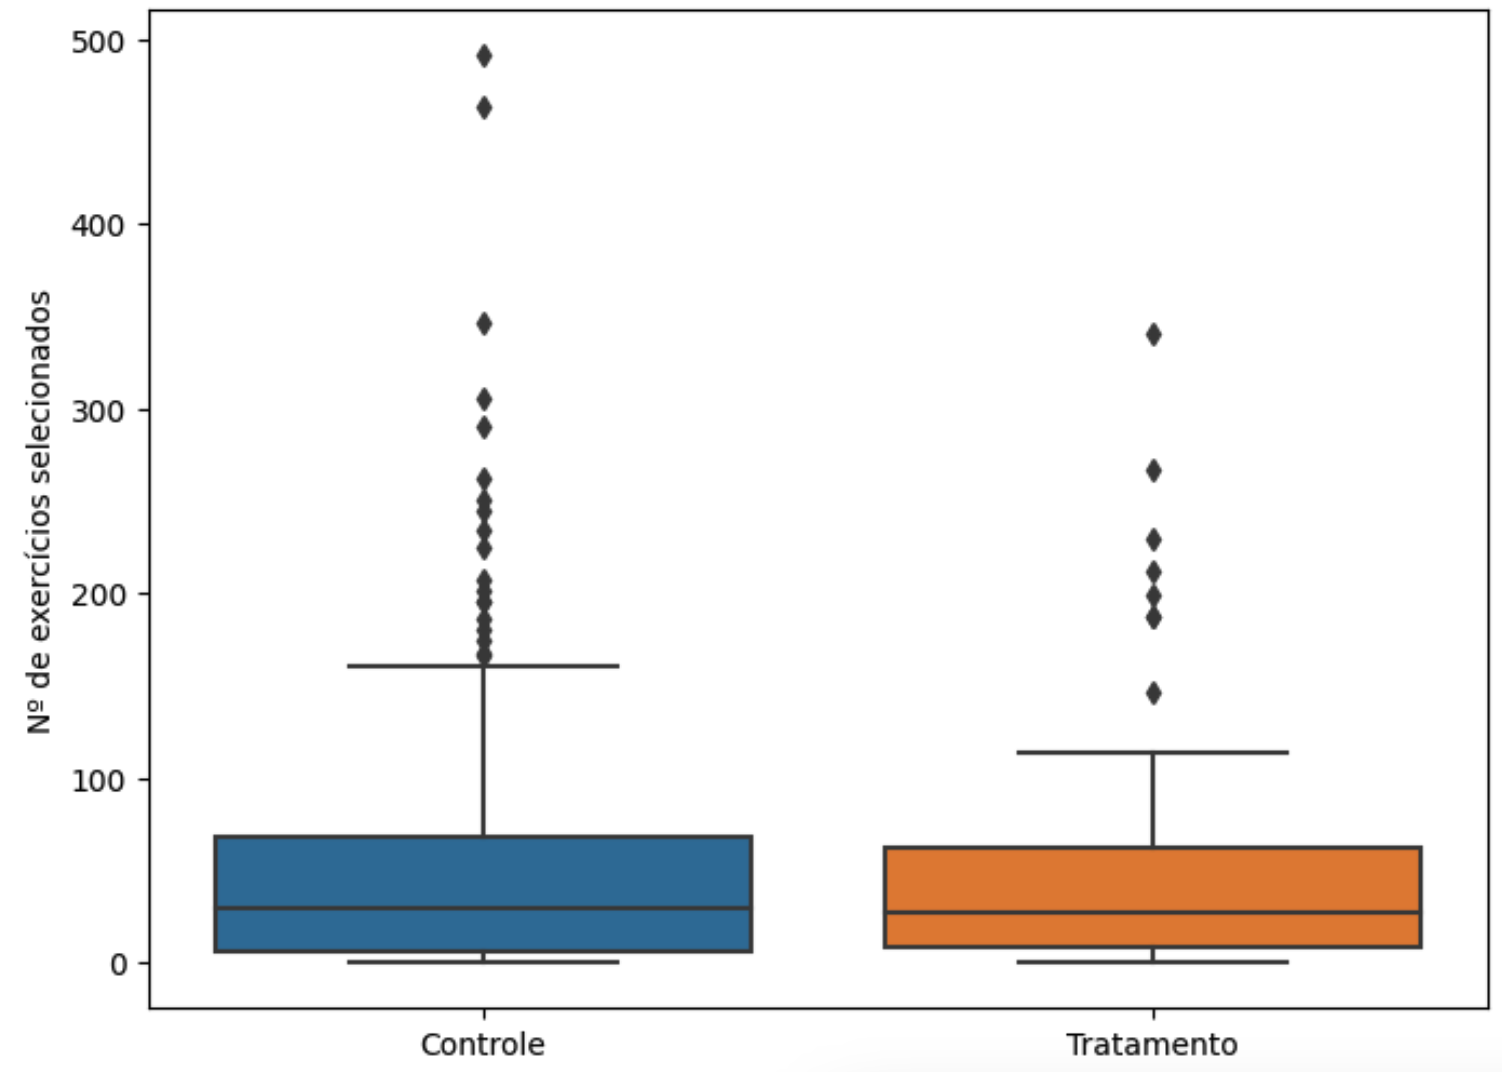
\includegraphics[width=0.85\linewidth]{figuras/boxplot_exs_before.png}
    \begin{center}
        \text{Fonte: Autor}
    \end{center}
    \label{fig:box-exs-before}
\end{figure}

\begin{figure}
    \centering
    \caption{Gráfico de Caixa do Número de Exercícios Selecionados Após Remoção de \textit{Outliers}}
    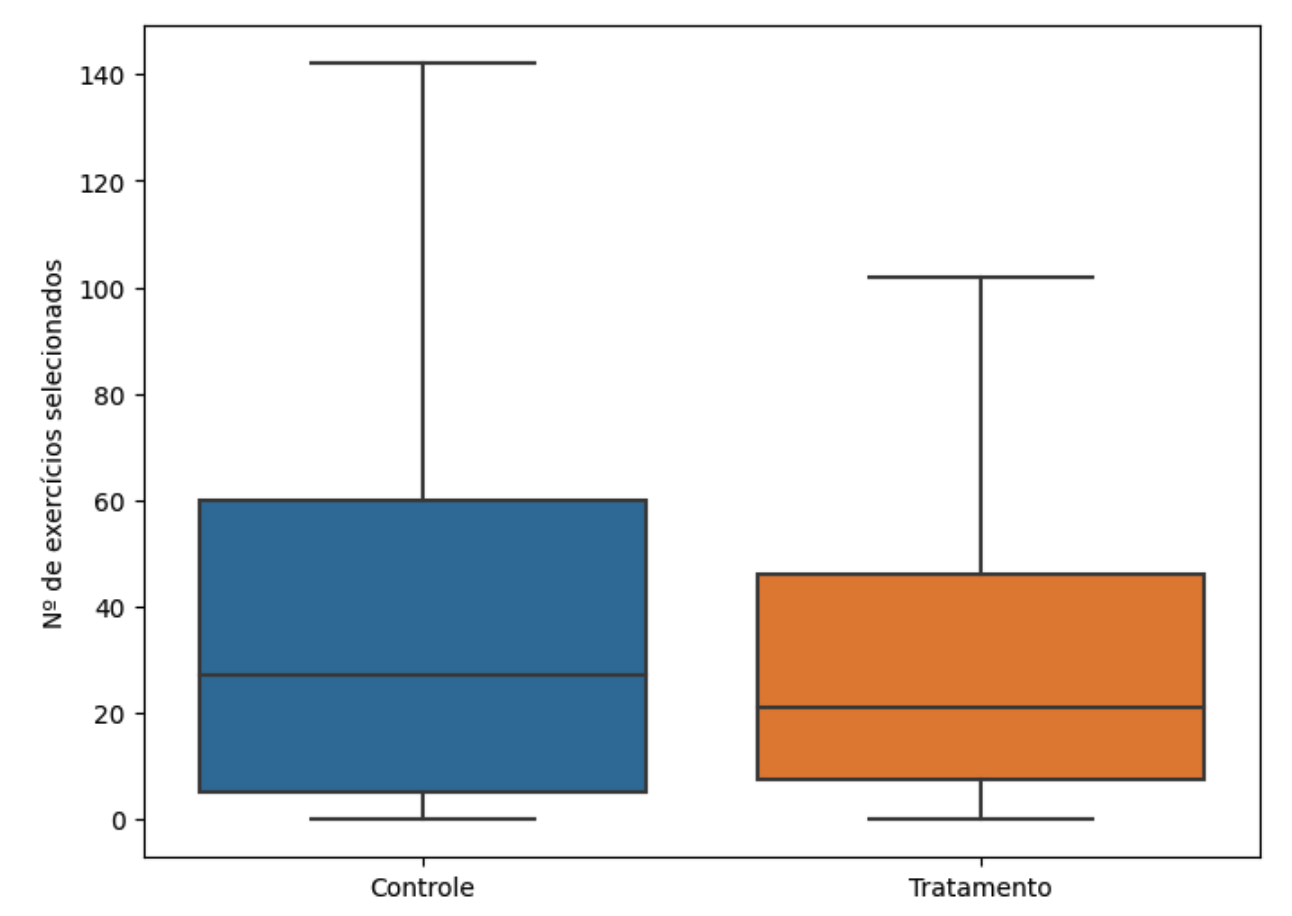
\includegraphics[width=0.85\linewidth]{figuras/boxplot_exs_after.png}
    \begin{center}
        \text{Fonte: Autor}
    \end{center}
    \label{fig:box-exs-after}
\end{figure}

\begin{figure}
    \centering
    \caption{Medidas de Tendência Central do Número de Exercícios Selecionados Antes da Remoção de \textit{Outliers}}
    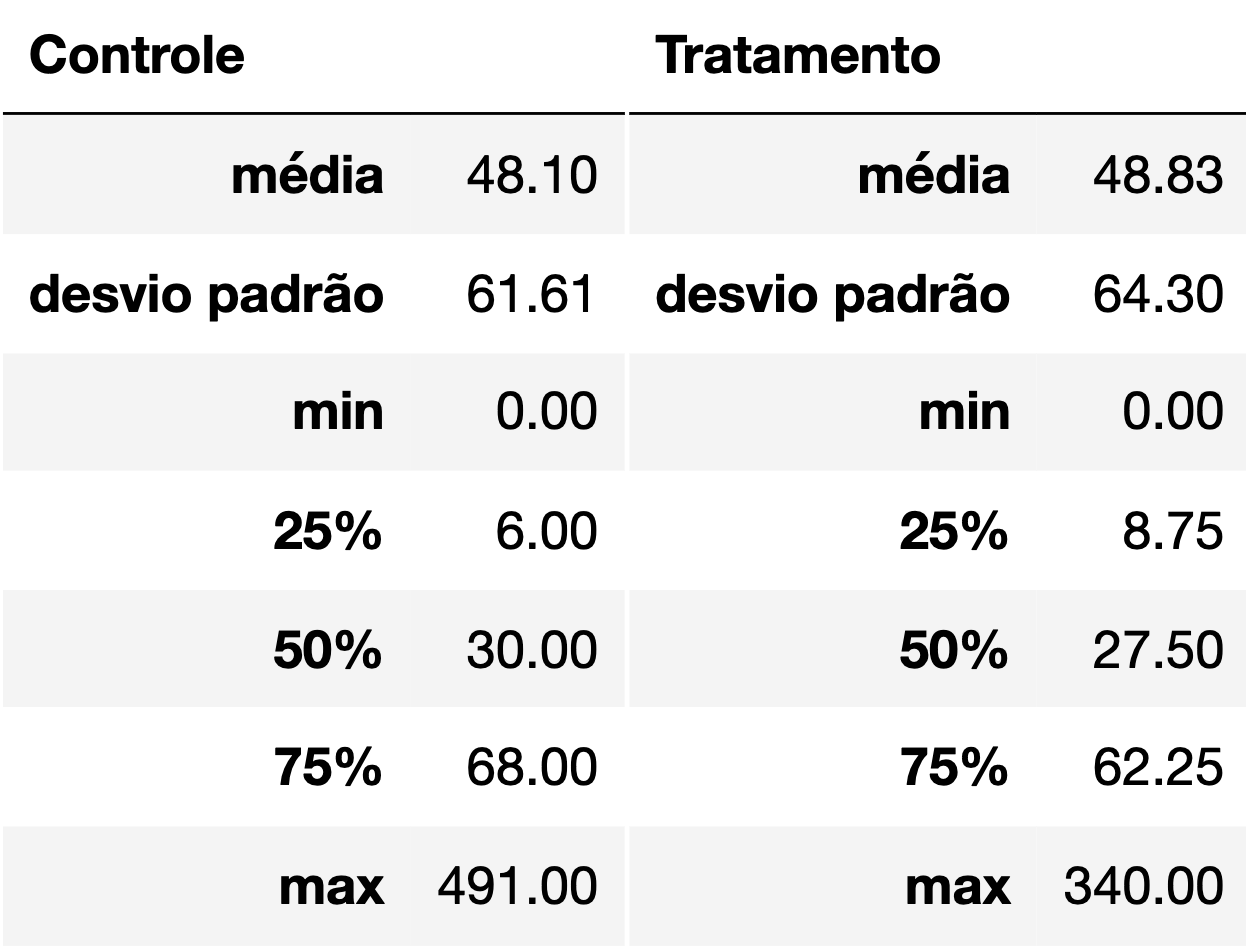
\includegraphics[width=0.45\linewidth]{figuras/mtc_exs_before.png}
    \begin{center}
        \text{Fonte: Autor}
    \end{center}
    \label{fig:mtc-exs-before}
\end{figure}

\begin{figure}
    \centering
    \caption{Medidas de Tendência Central do Número de Exercícios Selecionados Após Remoção de \textit{Outliers}}
    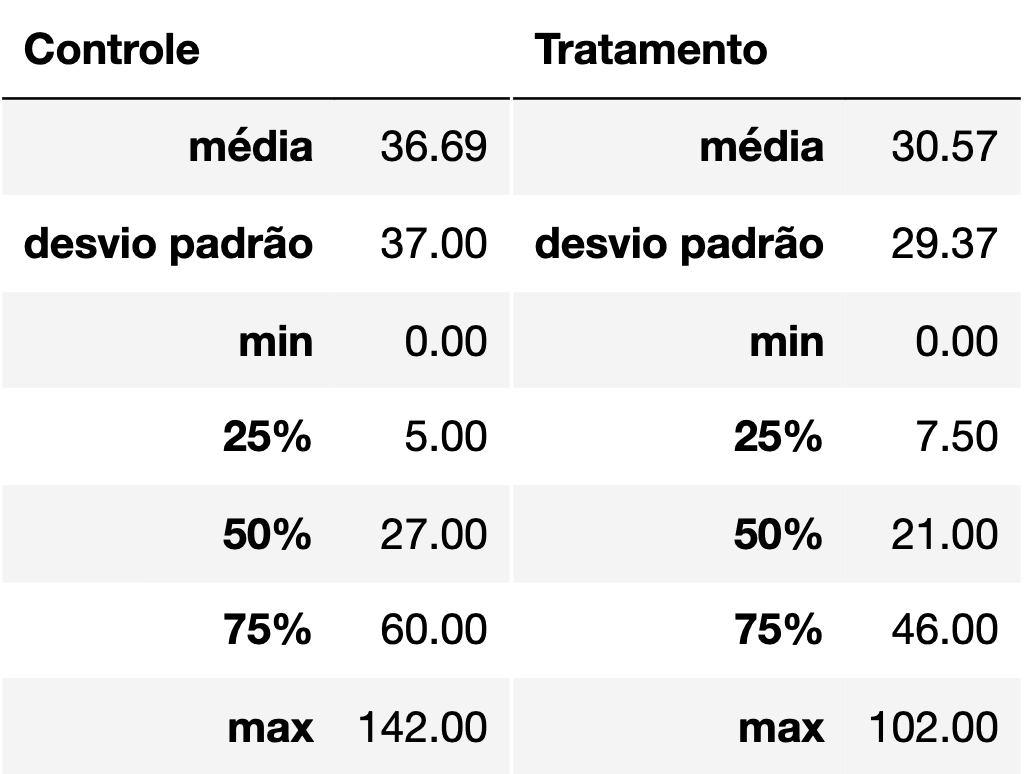
\includegraphics[width=0.45\linewidth]{figuras/mtc_exs_after.png}
    \begin{center}
        \text{Fonte: Autor}
    \end{center}
    \label{fig:mtc-exs-after}
\end{figure}

A remoção dos \textit{outliers} foi uma etapa essencial para garantir a precisão da análise estatística. Embora esses pontos de dados não sejam inválidos, sua grande discrepância em relação ao restante do conjunto poderia enviesar os cálculos dos indicadores de qualidade em uso. Após essa etapa, procedeu-se à normalização das métricas, utilizando a combinação dos métodos de máximo e mínimo com a transformação \textit{Box-Cox}.

A escolha do método \textit{Box-Cox} foi motivada pela necessidade de tratar distribuições assimétricas positivamente, como observado nos gráficos de caixa apresentados anteriormente. Além disso, a normalização pelo método de máximo e mínimo garantiu que todas as métricas fossem convertidas para valores no intervalo entre 0 e 1, o que é necessário o cálculo do indicador agregado de qualidade em uso (estes procedimentos são detalhados na Subseção \ref{subsec:normalization}).

Finalizados os procedimentos de análise de estatística descritiva, redução e normalização dos dados, calculou-se o indicador único de qualidade em uso para cada usuário, utilizando os pesos definidos na subseção anterior:

\[
Q = 0.8333(f) + 0.1667(0.8889(l) + 0.1111(e)),
\]

onde \textit{Q} representa o indicador final, \textit{f} corresponde ao número normalizado de usos do filtro, \textit{l} ao número normalizado de listas criadas, e \textit{e} à quantidade de exercícios selecionados. Cada usuário, portanto, recebeu um valor único entre 0 e 1, refletindo sua percepção da qualidade em uso da funcionalidade. A distribuição dos valores obtidos para os grupos de controle e tratamento pode ser observada na Figura \ref{fig:scores-dist}, enquanto as medidas de tendência central desses indicadores são apresentadas na Figura \ref{fig:mtc-scores}.

\begin{figure}
    \centering
    \caption{Distribuições dos Indicadores de Qualidade em Uso Percebida}
    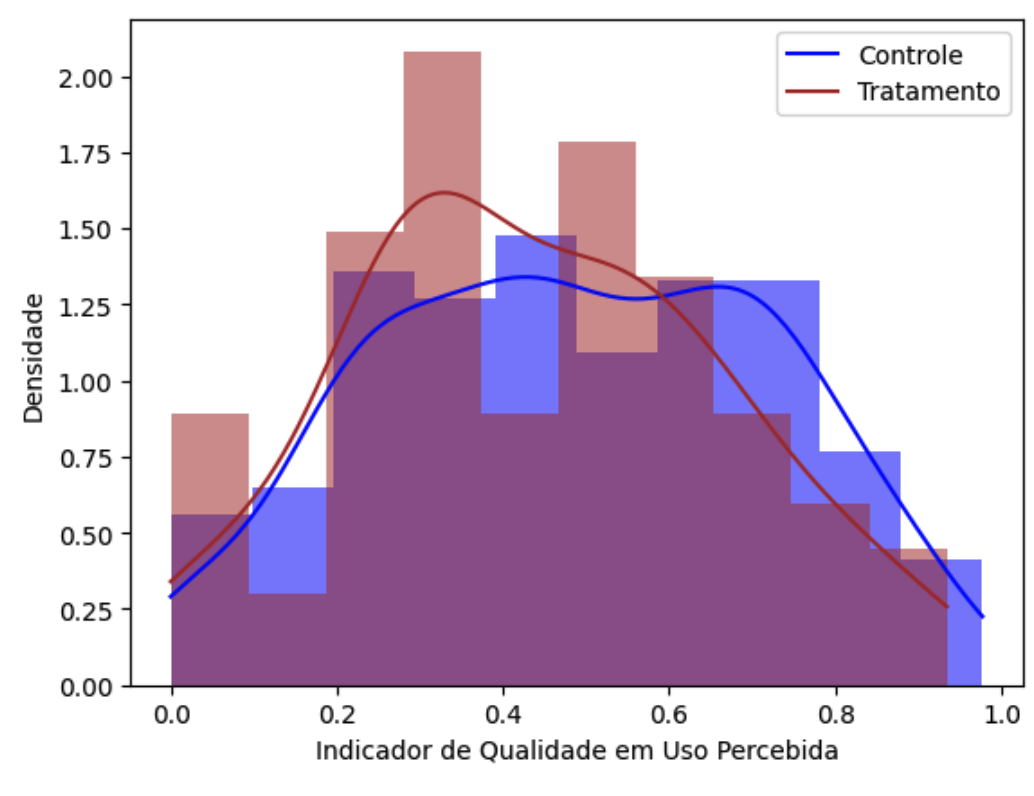
\includegraphics[width=0.85\linewidth]{figuras/scores_dist.png}
    \begin{center}
        \text{Fonte: Autor}
    \end{center}
    \label{fig:scores-dist}
\end{figure}

\begin{figure}
    \centering
    \caption{Medidas de Tendência Central dos Indicadores de Qualidade em Uso Percebida}
    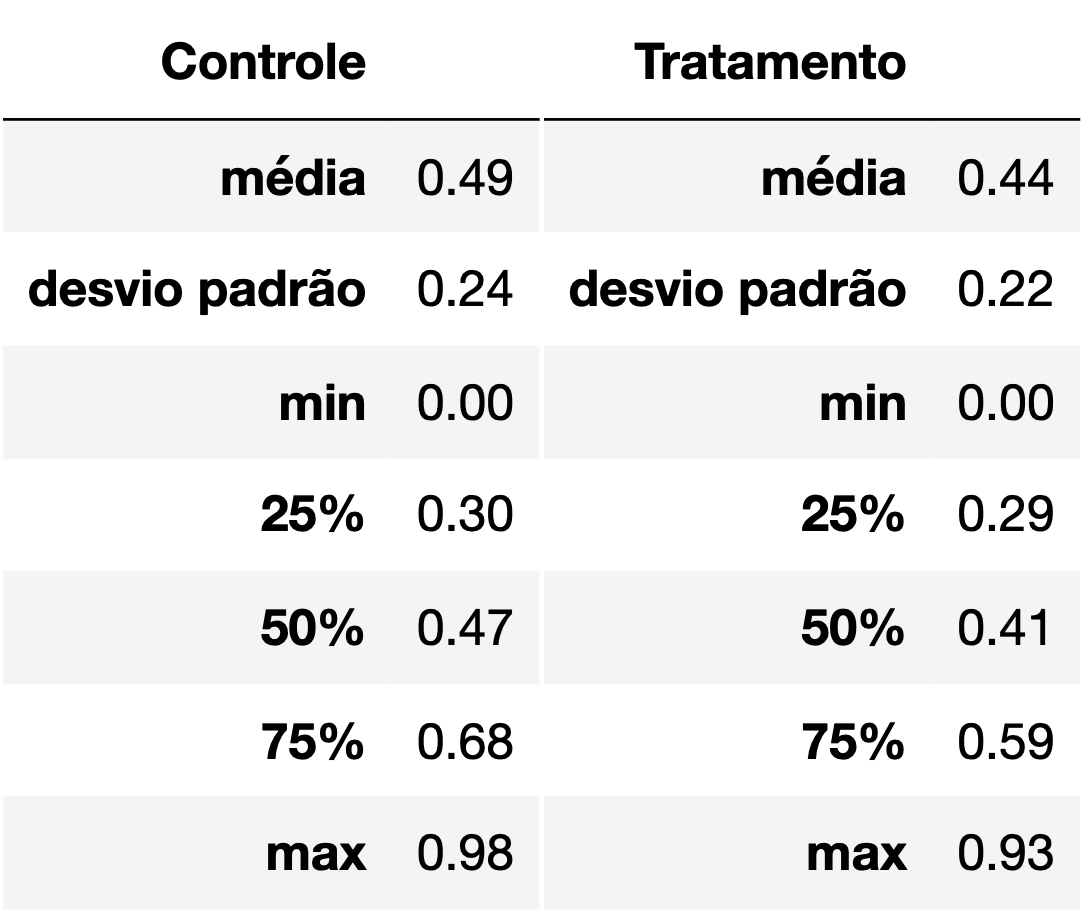
\includegraphics[width=0.45\linewidth]{figuras/mtc_scores.png}
    \begin{center}
        \text{Fonte: Autor}
    \end{center}
    \label{fig:mtc-scores}
\end{figure}

Após a realização das análises estatísticas descritivas dos conjuntos de indicadores calculados, foi aplicado o teste de Mann-Whitney U para comparar os grupos. Considerando um nível de significância de 5\%, não foi identificada diferença estatisticamente significativa entre os valores encontrados nas populações analisadas (U=13923 e p$\approx$ 0.13). Esse resultado indica que \textbf{não foi possível detectar uma diferença na qualidade em uso entre as versões de controle e de tratamento} \footnote{Os dados coletados foram anonimizados e disponibilizados em repositório público, juntamente com todas as análises realizadas. Endereço: \href{https://github.com/senaarth/tcc-notebooks/blob/main/experiment.ipynb}{https://github.com/senaarth/tcc-notebooks}}.

Diante da ausência de diferenças significativas na qualidade em uso entre as versões, foram conduzidas análises adicionais para servir de insumos para a tomada de decisão da equipe. Com base na suposição inicial que motivou este experimento, foram realizados testes para avaliar a frequência de adoção da funcionalidade de filtro por nível de dificuldade entre os grupos. Para isso, a partir dos eventos de uso do filtro, foi contabilizado o número de usuários que utilizaram ao menos uma vez o filtro da categoria em questão. Por se tratar de um dado categórico, optou-se pela aplicação do teste qui-quadrado para verificar a existência de uma diferença estatisticamente significativa entre os grupos.

Ao considerar a amostra total, composta por 3504 usuários (sendo 508, 14.5\%, do grupo de tratamento e 2996, 85.5\%, do grupo de controle), o teste qui-quadrado resultou em um p-valor de aproximadamente 0.0896 e um valor da estatística qui-quadrado de 2.88. Esses resultados indicam que, para um nível de confiança de 5\%, não haviam evidências estatísticas suficientes para afirmar diferença na funcionalidade entre os grupos analisados. No entanto, apesar do p-valor estar ligeiramente acima do limite de significância definido, ele ainda se encontrava em uma faixa próxima ao limiar. Dessa forma, para minimizar a possibilidade de um erro do tipo II, foi conduzida uma nova iteração do experimento, com uma extensão do período de coleta de dados por mais duas semanas (de 19 de novembro a 3 de dezembro de 2024).

Ao final do novo período de coleta, o teste foi reaplicado com uma amostra ampliada, agora composta por 4467 usuários, sendo 608 (13.6\%) pertencentes ao grupo de tratamento e 3859 (86.4\%) ao grupo de controle. Os novos resultados indicaram uma diferença estatisticamente significativa na adoção da funcionalidade entre os grupos, com um p-valor de aproximadamente 0.0032 e uma estatística qui-quadrado de 8.71 (ver Figura \ref{fig:exp-adocao-dificuldade}). Esse achado indicou que a alteração na posição do filtro influenciou sua adoção pelos usuários.

Por fim, visando se confirmar a suspeita de que a categoria posicionada por último seria a menos utilizada, foi realizado o mesmo teste, porém olhando para a categoria de fonte (esta, na versão de tratamento, se tornou a última). Os resultados apresentaram que sua proporção de adoção também foi maior na população de controle, contradizendo as suposições iniciais da equipe (U$\approx$3.92 e p$\approx$0.47, ver Figura \ref{fig:exp-adocao-fonte}).



\begin{figure}
    \centering
    \caption{Teste Sobre Adoção do Filtro de Nível de Dificuldade no Experimento}
    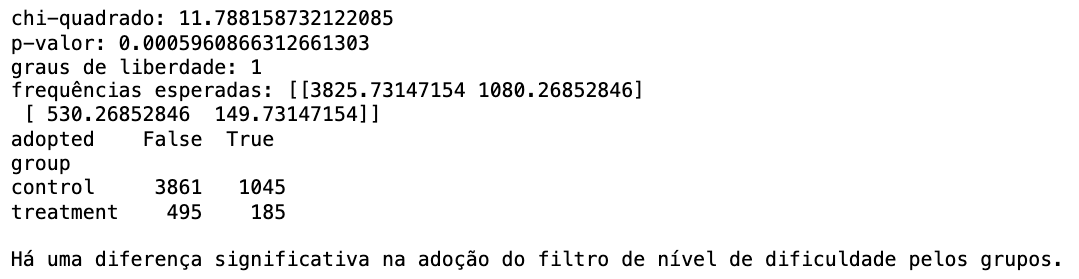
\includegraphics[width=0.85\linewidth]{figuras/adocao_dificuldade_experimento.png}
    \begin{center}
        \text{Fonte: Autor}
    \end{center}
    \label{fig:exp-adocao-dificuldade}
\end{figure}



\begin{figure}
    \centering
    \caption{Teste Sobre Adoção do Filtro de Fonte no Experimento}
    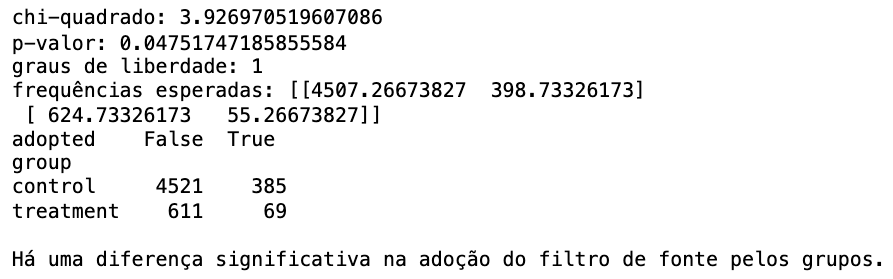
\includegraphics[width=0.85\linewidth]{figuras/adocao_fonte_experimento.png}
    \begin{center}
        \text{Fonte: Autor}
    \end{center}
    \label{fig:exp-adocao-fonte}
\end{figure}